%!TEX root = main.tex

\begin{figure*}[tbp]
	\newcommand\mywidth{0.19}
	\centering
	\subfloat[] {
		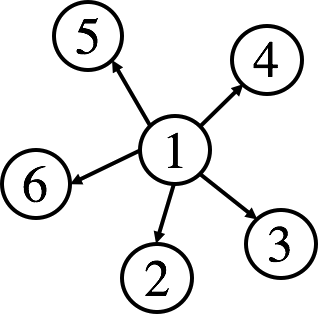
\includegraphics[width=0.14\textwidth,valign=c]{observcas}
		\vphantom{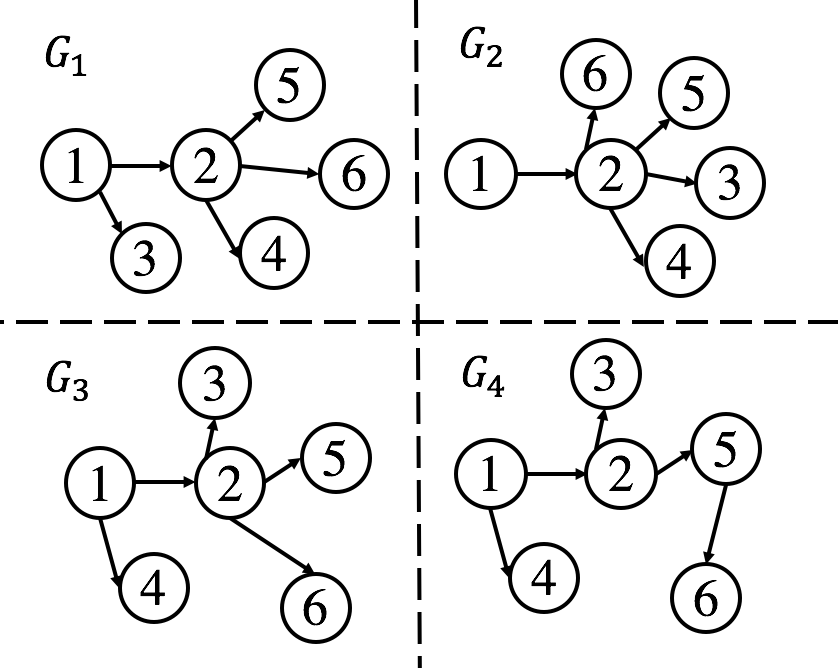
\includegraphics[height=\mywidth\textheight,valign=c]{somepossicas}}% MAR: this is here to keep the label at the same position as for the other figures.
		\label{fig:side:a}
	}
	\hspace{0.15cm}
	\subfloat[] {
		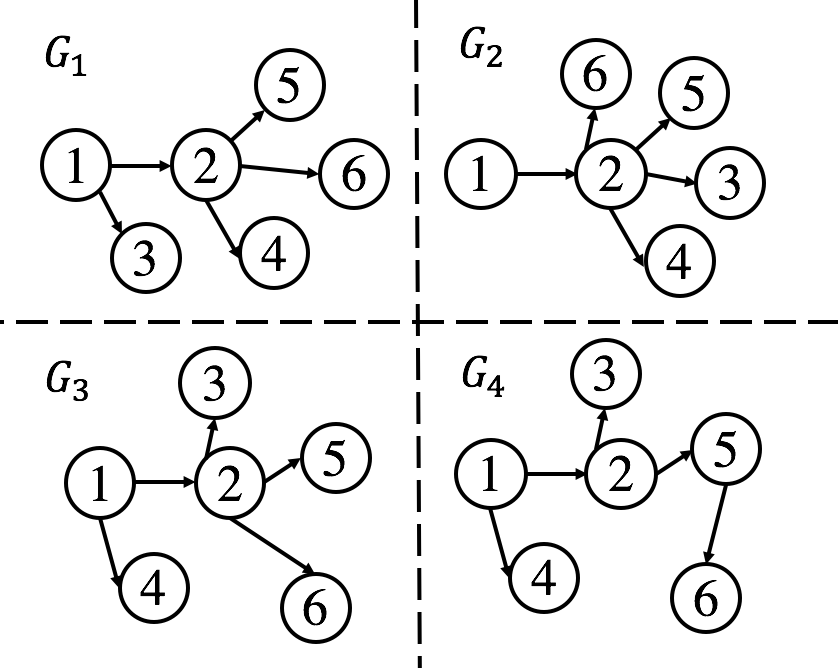
\includegraphics[height=\mywidth\textheight,valign=c]{somepossicas}
		\label{fig:side:b}
	}
	\hspace{0.15cm}
	\subfloat[] {
		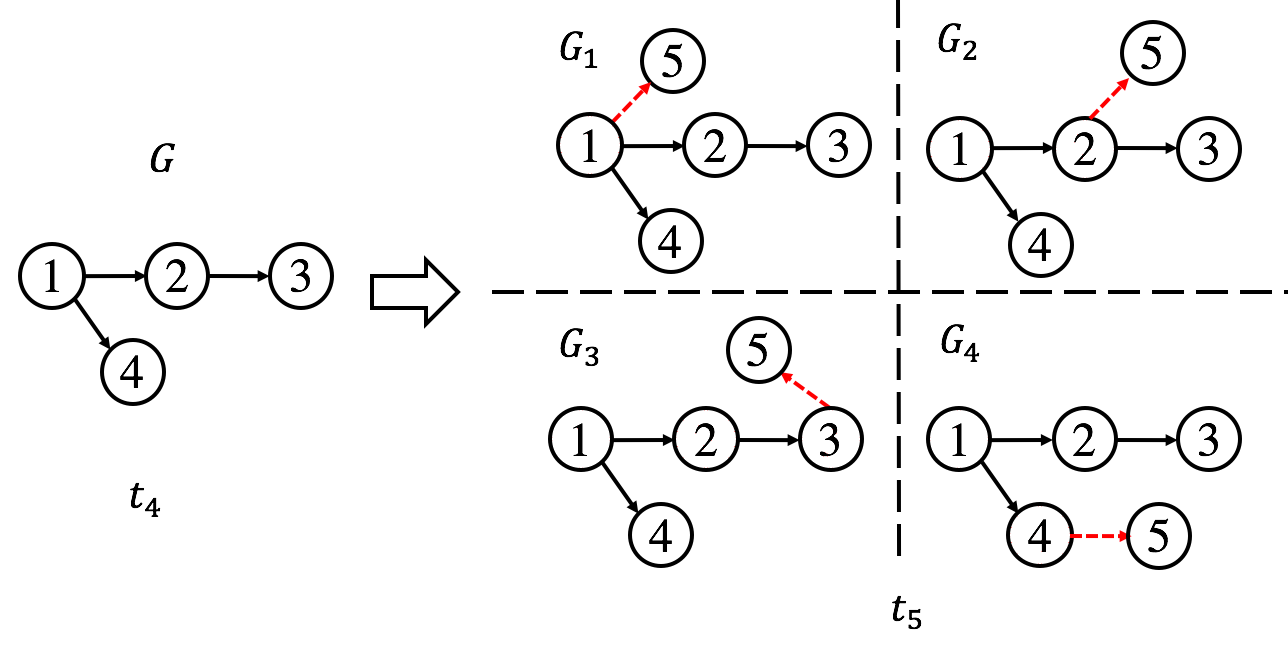
\includegraphics[height=\mywidth\textheight,valign=c]{gen_col}
		\label{fig:add-one-edge}
	}
	\caption{ 
		Modeling latent diffusions.
		\textbf{(a)} The schema of a retweet cascade as provided by the Twitter API, in which all retweets are attributed to the original tweet.
		\textbf{(b)} Four diffusion scenarios (out of 120 possible scenarios), associated with the retweet cascade in (a).
		\textbf{(c)} Intuition of the independent conditional model.
		A new node $v_5$ appears conditioned on one diffusion scenario $G$.
		Four new diffusion scenarios are generated as $v_5$ can attach to any of the existing nodes.
%		\hl{The influence of each of the nodes colored in red increases as $v_5$ attaches.}\verify{LX: unclear what ``increases'' refers to. suggest removing the red coloring and the sentence. i.e. this caption works equally well without the two highlighted sentences.}
	}
	\label{fig:holdout-ll}
%	\captionmoveup
\end{figure*}